\chapter{p3 = 35 (14 graphs)}
\newpage\begin{figure}
  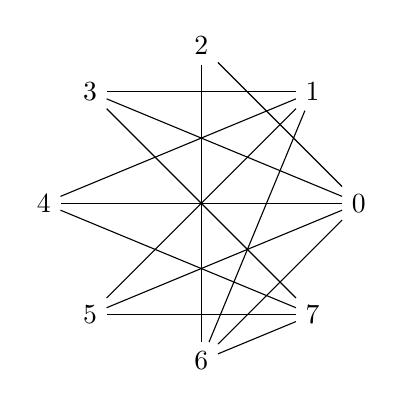
\begin{tikzpicture}
      \draw
        (0.0:2) node (0){0}
        (45.0:2) node (1){1}
        (90.0:2) node (2){2}
        (135.0:2) node (3){3}
        (180.0:2) node (4){4}
        (225.0:2) node (5){5}
        (270.0:2) node (6){6}
        (315.0:2) node (7){7};
      \begin{scope}[-]
        \draw (0) to (2);
        \draw (0) to (3);
        \draw (0) to (4);
        \draw (0) to (5);
        \draw (0) to (6);
        \draw (1) to (3);
        \draw (1) to (4);
        \draw (1) to (5);
        \draw (1) to (6);
        \draw (2) to (6);
        \draw (3) to (7);
        \draw (4) to (7);
        \draw (5) to (7);
        \draw (6) to (7);
      \end{scope}
    \end{tikzpicture}
\end{figure}
\begin{itemize}
\item signature: 0111110011110000100001001011
\item g: Graph with 8 nodes and 14 edges
\item order: 8
\item size: 14
\item max degree: 5
\item degrees: 2,3,3,3,4,4,4,5
\item is tree: 0
\item is bipartite: 0
\item has bridge: 0
\item is chordal: 0
\item is complete: 0
\item min cycle basis weight: 27
\item min cycle basis size: 7
\item diameter: 2
\item radius: 2
\item is eulerian: 0
\item is planar: 0
\item number of faces: 8
\item is regular: 0
\item p3: 35
\item p4: None
\item property hash: 4e556e1cc948fcc221fdd5f077a15b8a03269cf83ebc7fab35317b9fdb979903
\end{itemize}
\newpage
\begin{figure}
  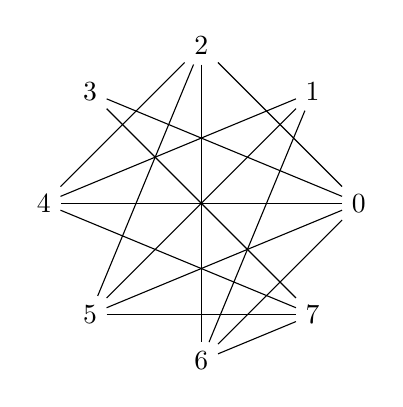
\begin{tikzpicture}
      \draw
        (0.0:2) node (0){0}
        (45.0:2) node (1){1}
        (90.0:2) node (2){2}
        (135.0:2) node (3){3}
        (180.0:2) node (4){4}
        (225.0:2) node (5){5}
        (270.0:2) node (6){6}
        (315.0:2) node (7){7};
      \begin{scope}[-]
        \draw (0) to (2);
        \draw (0) to (3);
        \draw (0) to (4);
        \draw (0) to (5);
        \draw (0) to (6);
        \draw (1) to (4);
        \draw (1) to (5);
        \draw (1) to (6);
        \draw (2) to (4);
        \draw (2) to (5);
        \draw (2) to (6);
        \draw (3) to (7);
        \draw (4) to (7);
        \draw (5) to (7);
        \draw (6) to (7);
      \end{scope}
    \end{tikzpicture}
\end{figure}
\begin{itemize}
\item signature: 0111110001110011100001001011
\item g: Graph with 8 nodes and 15 edges
\item order: 8
\item size: 15
\item max degree: 5
\item degrees: 2,3,4,4,4,4,4,5
\item is tree: 0
\item is bipartite: 0
\item has bridge: 0
\item is chordal: 0
\item is complete: 0
\item min cycle basis weight: 29
\item min cycle basis size: 8
\item diameter: 3
\item radius: 2
\item is eulerian: 0
\item is planar: 0
\item number of faces: 9
\item is regular: 0
\item p3: 35
\item p4: 10
\item property hash: 1c6c46c0e50494e18b11d9f6c490eedb75dc53084e1d11dc4fd18fb78495a75d
\end{itemize}
\newpage
\begin{figure}
  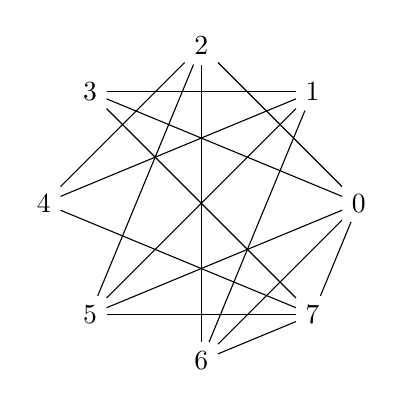
\begin{tikzpicture}
      \draw
        (0.0:2) node (0){0}
        (45.0:2) node (1){1}
        (90.0:2) node (2){2}
        (135.0:2) node (3){3}
        (180.0:2) node (4){4}
        (225.0:2) node (5){5}
        (270.0:2) node (6){6}
        (315.0:2) node (7){7};
      \begin{scope}[-]
        \draw (0) to (2);
        \draw (0) to (3);
        \draw (0) to (5);
        \draw (0) to (6);
        \draw (0) to (7);
        \draw (1) to (3);
        \draw (1) to (4);
        \draw (1) to (5);
        \draw (1) to (6);
        \draw (2) to (4);
        \draw (2) to (5);
        \draw (2) to (6);
        \draw (3) to (7);
        \draw (4) to (7);
        \draw (5) to (7);
        \draw (6) to (7);
      \end{scope}
    \end{tikzpicture}
\end{figure}
\begin{itemize}
\item signature: 0110111011110011100001001011
\item g: Graph with 8 nodes and 16 edges
\item order: 8
\item size: 16
\item max degree: 5
\item degrees: 3,3,4,4,4,4,5,5
\item is tree: 0
\item is bipartite: 0
\item has bridge: 0
\item is chordal: 0
\item is complete: 0
\item min cycle basis weight: 31
\item min cycle basis size: 9
\item diameter: 2
\item radius: 2
\item is eulerian: 0
\item is planar: 0
\item number of faces: 10
\item is regular: 0
\item p3: 35
\item p4: 13
\item property hash: 0c5b0c04357491c714e6d7646d4856119931539a594895c9cbc1bf7da0bad65f
\end{itemize}
\newpage
\begin{figure}
  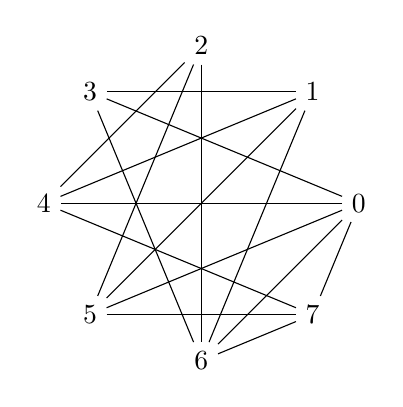
\begin{tikzpicture}
      \draw
        (0.0:2) node (0){0}
        (45.0:2) node (1){1}
        (90.0:2) node (2){2}
        (135.0:2) node (3){3}
        (180.0:2) node (4){4}
        (225.0:2) node (5){5}
        (270.0:2) node (6){6}
        (315.0:2) node (7){7};
      \begin{scope}[-]
        \draw (0) to (3);
        \draw (0) to (4);
        \draw (0) to (5);
        \draw (0) to (6);
        \draw (0) to (7);
        \draw (1) to (3);
        \draw (1) to (4);
        \draw (1) to (5);
        \draw (1) to (6);
        \draw (2) to (4);
        \draw (2) to (5);
        \draw (2) to (6);
        \draw (3) to (6);
        \draw (4) to (7);
        \draw (5) to (7);
        \draw (6) to (7);
      \end{scope}
    \end{tikzpicture}
\end{figure}
\begin{itemize}
\item signature: 0011111011110011100010001011
\item g: Graph with 8 nodes and 16 edges
\item order: 8
\item size: 16
\item max degree: 5
\item degrees: 3,3,4,4,4,4,5,5
\item is tree: 0
\item is bipartite: 0
\item has bridge: 0
\item is chordal: 0
\item is complete: 0
\item min cycle basis weight: 31
\item min cycle basis size: 9
\item diameter: 2
\item radius: 2
\item is eulerian: 0
\item is planar: 0
\item number of faces: 10
\item is regular: 0
\item p3: 35
\item p4: None
\item property hash: b921b19b731f1e6aed68d6227eddd0bad22a483d8d3106e010b5896eb680f7d2
\end{itemize}
\newpage
\begin{figure}
  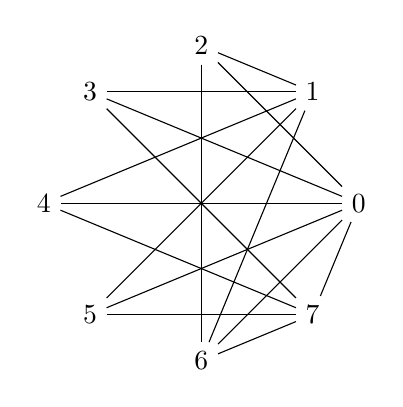
\begin{tikzpicture}
      \draw
        (0.0:2) node (0){0}
        (45.0:2) node (1){1}
        (90.0:2) node (2){2}
        (135.0:2) node (3){3}
        (180.0:2) node (4){4}
        (225.0:2) node (5){5}
        (270.0:2) node (6){6}
        (315.0:2) node (7){7};
      \begin{scope}[-]
        \draw (0) to (2);
        \draw (0) to (3);
        \draw (0) to (4);
        \draw (0) to (5);
        \draw (0) to (6);
        \draw (0) to (7);
        \draw (1) to (2);
        \draw (1) to (3);
        \draw (1) to (4);
        \draw (1) to (5);
        \draw (1) to (6);
        \draw (2) to (6);
        \draw (3) to (7);
        \draw (4) to (7);
        \draw (5) to (7);
        \draw (6) to (7);
      \end{scope}
    \end{tikzpicture}
\end{figure}
\begin{itemize}
\item signature: 0111111111110000100001001011
\item g: Graph with 8 nodes and 16 edges
\item order: 8
\item size: 16
\item max degree: 6
\item degrees: 3,3,3,3,4,5,5,6
\item is tree: 0
\item is bipartite: 0
\item has bridge: 0
\item is chordal: 0
\item is complete: 0
\item min cycle basis weight: 30
\item min cycle basis size: 9
\item diameter: 2
\item radius: 2
\item is eulerian: 0
\item is planar: 0
\item number of faces: 10
\item is regular: 0
\item p3: 35
\item p4: None
\item property hash: bfdc339b84b247890bdbba8bf8058d7587eb699d804ae7fd205caba41c005093
\end{itemize}
\newpage
\begin{figure}
  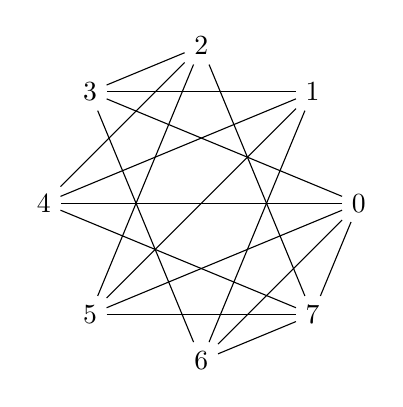
\begin{tikzpicture}
      \draw
        (0.0:2) node (0){0}
        (45.0:2) node (1){1}
        (90.0:2) node (2){2}
        (135.0:2) node (3){3}
        (180.0:2) node (4){4}
        (225.0:2) node (5){5}
        (270.0:2) node (6){6}
        (315.0:2) node (7){7};
      \begin{scope}[-]
        \draw (0) to (3);
        \draw (0) to (4);
        \draw (0) to (5);
        \draw (0) to (6);
        \draw (0) to (7);
        \draw (1) to (3);
        \draw (1) to (4);
        \draw (1) to (5);
        \draw (1) to (6);
        \draw (2) to (3);
        \draw (2) to (4);
        \draw (2) to (5);
        \draw (2) to (7);
        \draw (3) to (6);
        \draw (4) to (7);
        \draw (5) to (7);
        \draw (6) to (7);
      \end{scope}
    \end{tikzpicture}
\end{figure}
\begin{itemize}
\item signature: 0011111011110111010010001011
\item g: Graph with 8 nodes and 17 edges
\item order: 8
\item size: 17
\item max degree: 5
\item degrees: 4,4,4,4,4,4,5,5
\item is tree: 0
\item is bipartite: 0
\item has bridge: 0
\item is chordal: 0
\item is complete: 0
\item min cycle basis weight: 33
\item min cycle basis size: 10
\item diameter: 2
\item radius: 2
\item is eulerian: 0
\item is planar: 0
\item number of faces: 11
\item is regular: 0
\item p3: 35
\item p4: 13
\item property hash: f9e7ec33ba54e3c232da2a864b51ea2a36ef4711fe296170daa55fe0ac0a2df4
\end{itemize}
\newpage
\begin{figure}
  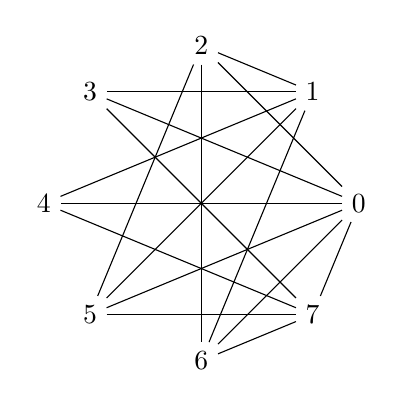
\begin{tikzpicture}
      \draw
        (0.0:2) node (0){0}
        (45.0:2) node (1){1}
        (90.0:2) node (2){2}
        (135.0:2) node (3){3}
        (180.0:2) node (4){4}
        (225.0:2) node (5){5}
        (270.0:2) node (6){6}
        (315.0:2) node (7){7};
      \begin{scope}[-]
        \draw (0) to (2);
        \draw (0) to (3);
        \draw (0) to (4);
        \draw (0) to (5);
        \draw (0) to (6);
        \draw (0) to (7);
        \draw (1) to (2);
        \draw (1) to (3);
        \draw (1) to (4);
        \draw (1) to (5);
        \draw (1) to (6);
        \draw (2) to (5);
        \draw (2) to (6);
        \draw (3) to (7);
        \draw (4) to (7);
        \draw (5) to (7);
        \draw (6) to (7);
      \end{scope}
    \end{tikzpicture}
\end{figure}
\begin{itemize}
\item signature: 0111111111110001100001001011
\item g: Graph with 8 nodes and 17 edges
\item order: 8
\item size: 17
\item max degree: 6
\item degrees: 3,3,4,4,4,5,5,6
\item is tree: 0
\item is bipartite: 0
\item has bridge: 0
\item is chordal: 0
\item is complete: 0
\item min cycle basis weight: 32
\item min cycle basis size: 10
\item diameter: 2
\item radius: 2
\item is eulerian: 0
\item is planar: 0
\item number of faces: 11
\item is regular: 0
\item p3: 35
\item p4: None
\item property hash: 4c9bf8d9a49592b51751c4c5d73aa04b5dae261c8a3e209d4b9622a379127ae4
\end{itemize}
\newpage
\begin{figure}
  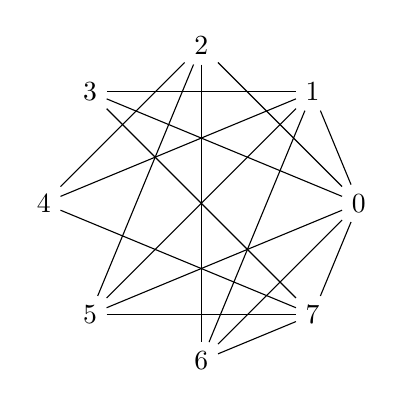
\begin{tikzpicture}
      \draw
        (0.0:2) node (0){0}
        (45.0:2) node (1){1}
        (90.0:2) node (2){2}
        (135.0:2) node (3){3}
        (180.0:2) node (4){4}
        (225.0:2) node (5){5}
        (270.0:2) node (6){6}
        (315.0:2) node (7){7};
      \begin{scope}[-]
        \draw (0) to (1);
        \draw (0) to (2);
        \draw (0) to (3);
        \draw (0) to (5);
        \draw (0) to (6);
        \draw (0) to (7);
        \draw (1) to (3);
        \draw (1) to (4);
        \draw (1) to (5);
        \draw (1) to (6);
        \draw (2) to (4);
        \draw (2) to (5);
        \draw (2) to (6);
        \draw (3) to (7);
        \draw (4) to (7);
        \draw (5) to (7);
        \draw (6) to (7);
      \end{scope}
    \end{tikzpicture}
\end{figure}
\begin{itemize}
\item signature: 1110111011110011100001001011
\item g: Graph with 8 nodes and 17 edges
\item order: 8
\item size: 17
\item max degree: 6
\item degrees: 3,3,4,4,4,5,5,6
\item is tree: 0
\item is bipartite: 0
\item has bridge: 0
\item is chordal: 0
\item is complete: 0
\item min cycle basis weight: 32
\item min cycle basis size: 10
\item diameter: 2
\item radius: 2
\item is eulerian: 0
\item is planar: 0
\item number of faces: 11
\item is regular: 0
\item p3: 35
\item p4: None
\item property hash: 4c9bf8d9a49592b51751c4c5d73aa04b5dae261c8a3e209d4b9622a379127ae4
\end{itemize}
\newpage
\begin{figure}
  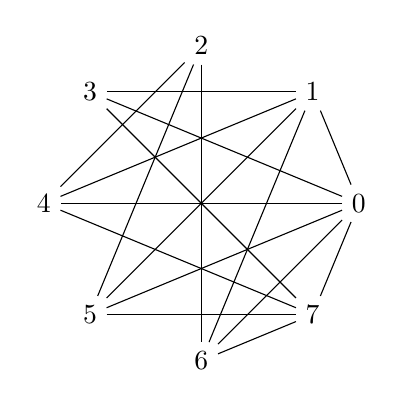
\begin{tikzpicture}
      \draw
        (0.0:2) node (0){0}
        (45.0:2) node (1){1}
        (90.0:2) node (2){2}
        (135.0:2) node (3){3}
        (180.0:2) node (4){4}
        (225.0:2) node (5){5}
        (270.0:2) node (6){6}
        (315.0:2) node (7){7};
      \begin{scope}[-]
        \draw (0) to (1);
        \draw (0) to (3);
        \draw (0) to (4);
        \draw (0) to (5);
        \draw (0) to (6);
        \draw (0) to (7);
        \draw (1) to (3);
        \draw (1) to (4);
        \draw (1) to (5);
        \draw (1) to (6);
        \draw (2) to (4);
        \draw (2) to (5);
        \draw (2) to (6);
        \draw (3) to (7);
        \draw (4) to (7);
        \draw (5) to (7);
        \draw (6) to (7);
      \end{scope}
    \end{tikzpicture}
\end{figure}
\begin{itemize}
\item signature: 1011111011110011100001001011
\item g: Graph with 8 nodes and 17 edges
\item order: 8
\item size: 17
\item max degree: 6
\item degrees: 3,3,4,4,4,5,5,6
\item is tree: 0
\item is bipartite: 0
\item has bridge: 0
\item is chordal: 0
\item is complete: 0
\item min cycle basis weight: 32
\item min cycle basis size: 10
\item diameter: 3
\item radius: 2
\item is eulerian: 0
\item is planar: 0
\item number of faces: 11
\item is regular: 0
\item p3: 35
\item p4: None
\item property hash: 67bcd16dce14a4c5545619d26380847fb62c9dfc7f23f3006e0fa9b6c63f3492
\end{itemize}
\newpage
\begin{figure}
  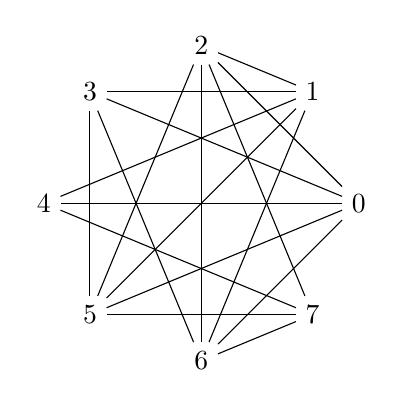
\begin{tikzpicture}
      \draw
        (0.0:2) node (0){0}
        (45.0:2) node (1){1}
        (90.0:2) node (2){2}
        (135.0:2) node (3){3}
        (180.0:2) node (4){4}
        (225.0:2) node (5){5}
        (270.0:2) node (6){6}
        (315.0:2) node (7){7};
      \begin{scope}[-]
        \draw (0) to (2);
        \draw (0) to (3);
        \draw (0) to (4);
        \draw (0) to (5);
        \draw (0) to (6);
        \draw (1) to (2);
        \draw (1) to (3);
        \draw (1) to (4);
        \draw (1) to (5);
        \draw (1) to (6);
        \draw (2) to (5);
        \draw (2) to (6);
        \draw (2) to (7);
        \draw (3) to (5);
        \draw (3) to (6);
        \draw (4) to (7);
        \draw (5) to (7);
        \draw (6) to (7);
      \end{scope}
    \end{tikzpicture}
\end{figure}
\begin{itemize}
\item signature: 0111110111110001110110001011
\item g: Graph with 8 nodes and 18 edges
\item order: 8
\item size: 18
\item max degree: 5
\item degrees: 3,4,4,5,5,5,5,5
\item is tree: 0
\item is bipartite: 0
\item has bridge: 0
\item is chordal: 0
\item is complete: 0
\item min cycle basis weight: 35
\item min cycle basis size: 11
\item diameter: 2
\item radius: 2
\item is eulerian: 0
\item is planar: 0
\item number of faces: 12
\item is regular: 0
\item p3: 35
\item p4: None
\item property hash: 36591247fe02676e896d1243de27bb11e40d238cb8364e7eed30832641b1a918
\end{itemize}
\newpage
\begin{figure}
  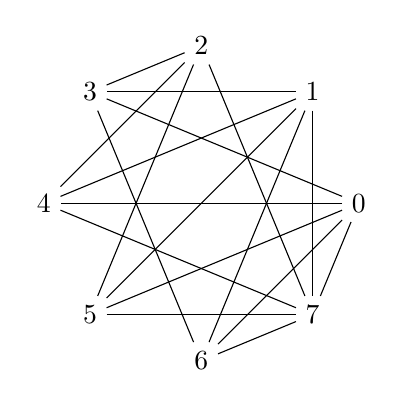
\begin{tikzpicture}
      \draw
        (0.0:2) node (0){0}
        (45.0:2) node (1){1}
        (90.0:2) node (2){2}
        (135.0:2) node (3){3}
        (180.0:2) node (4){4}
        (225.0:2) node (5){5}
        (270.0:2) node (6){6}
        (315.0:2) node (7){7};
      \begin{scope}[-]
        \draw (0) to (3);
        \draw (0) to (4);
        \draw (0) to (5);
        \draw (0) to (6);
        \draw (0) to (7);
        \draw (1) to (3);
        \draw (1) to (4);
        \draw (1) to (5);
        \draw (1) to (6);
        \draw (1) to (7);
        \draw (2) to (3);
        \draw (2) to (4);
        \draw (2) to (5);
        \draw (2) to (7);
        \draw (3) to (6);
        \draw (4) to (7);
        \draw (5) to (7);
        \draw (6) to (7);
      \end{scope}
    \end{tikzpicture}
\end{figure}
\begin{itemize}
\item signature: 0011111011111111010010001011
\item g: Graph with 8 nodes and 18 edges
\item order: 8
\item size: 18
\item max degree: 6
\item degrees: 4,4,4,4,4,5,5,6
\item is tree: 0
\item is bipartite: 0
\item has bridge: 0
\item is chordal: 0
\item is complete: 0
\item min cycle basis weight: 34
\item min cycle basis size: 11
\item diameter: 2
\item radius: 2
\item is eulerian: 0
\item is planar: 0
\item number of faces: 12
\item is regular: 0
\item p3: 35
\item p4: None
\item property hash: cfac93dc288628c854c38e966e5e01db61237941fb8ae340836f071ca473014a
\end{itemize}
\newpage
\begin{figure}
  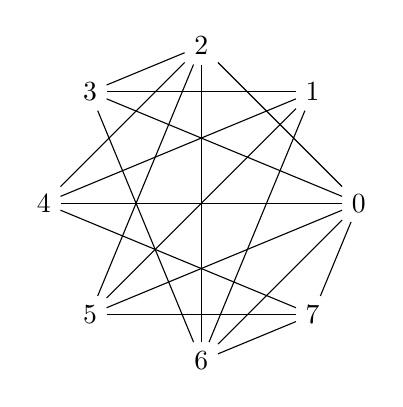
\begin{tikzpicture}
      \draw
        (0.0:2) node (0){0}
        (45.0:2) node (1){1}
        (90.0:2) node (2){2}
        (135.0:2) node (3){3}
        (180.0:2) node (4){4}
        (225.0:2) node (5){5}
        (270.0:2) node (6){6}
        (315.0:2) node (7){7};
      \begin{scope}[-]
        \draw (0) to (2);
        \draw (0) to (3);
        \draw (0) to (4);
        \draw (0) to (5);
        \draw (0) to (6);
        \draw (0) to (7);
        \draw (1) to (3);
        \draw (1) to (4);
        \draw (1) to (5);
        \draw (1) to (6);
        \draw (2) to (3);
        \draw (2) to (4);
        \draw (2) to (5);
        \draw (2) to (6);
        \draw (3) to (6);
        \draw (4) to (7);
        \draw (5) to (7);
        \draw (6) to (7);
      \end{scope}
    \end{tikzpicture}
\end{figure}
\begin{itemize}
\item signature: 0111111011110111100010001011
\item g: Graph with 8 nodes and 18 edges
\item order: 8
\item size: 18
\item max degree: 6
\item degrees: 4,4,4,4,4,5,5,6
\item is tree: 0
\item is bipartite: 0
\item has bridge: 0
\item is chordal: 0
\item is complete: 0
\item min cycle basis weight: 35
\item min cycle basis size: 11
\item diameter: 2
\item radius: 2
\item is eulerian: 0
\item is planar: 0
\item number of faces: 12
\item is regular: 0
\item p3: 35
\item p4: None
\item property hash: d718abfc761b890b2f6558f3e97e860e4d5c9072c977d406c069913ff7ac8831
\end{itemize}
\newpage
\begin{figure}
  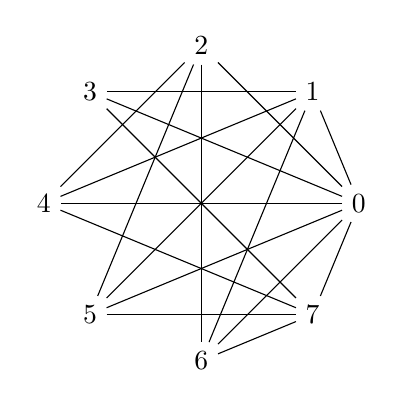
\begin{tikzpicture}
      \draw
        (0.0:2) node (0){0}
        (45.0:2) node (1){1}
        (90.0:2) node (2){2}
        (135.0:2) node (3){3}
        (180.0:2) node (4){4}
        (225.0:2) node (5){5}
        (270.0:2) node (6){6}
        (315.0:2) node (7){7};
      \begin{scope}[-]
        \draw (0) to (1);
        \draw (0) to (2);
        \draw (0) to (3);
        \draw (0) to (4);
        \draw (0) to (5);
        \draw (0) to (6);
        \draw (0) to (7);
        \draw (1) to (3);
        \draw (1) to (4);
        \draw (1) to (5);
        \draw (1) to (6);
        \draw (2) to (4);
        \draw (2) to (5);
        \draw (2) to (6);
        \draw (3) to (7);
        \draw (4) to (7);
        \draw (5) to (7);
        \draw (6) to (7);
      \end{scope}
    \end{tikzpicture}
\end{figure}
\begin{itemize}
\item signature: 1111111011110011100001001011
\item g: Graph with 8 nodes and 18 edges
\item order: 8
\item size: 18
\item max degree: 7
\item degrees: 3,4,4,4,4,5,5,7
\item is tree: 0
\item is bipartite: 0
\item has bridge: 0
\item is chordal: 0
\item is complete: 0
\item min cycle basis weight: 33
\item min cycle basis size: 11
\item diameter: 2
\item radius: 1
\item is eulerian: 0
\item is planar: 0
\item number of faces: 12
\item is regular: 0
\item p3: 35
\item p4: None
\item property hash: 9d9016aa97126b3c4ac3b373019af87264e80111afa22b3b02974002ac1c3a82
\end{itemize}
\newpage
\begin{figure}
  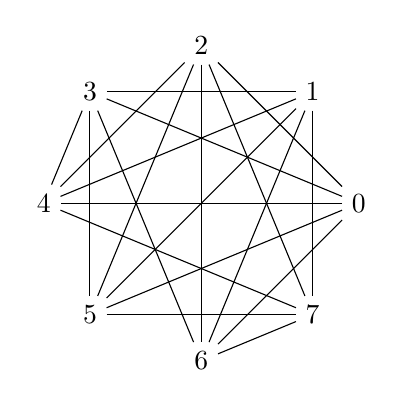
\begin{tikzpicture}
      \draw
        (0.0:2) node (0){0}
        (45.0:2) node (1){1}
        (90.0:2) node (2){2}
        (135.0:2) node (3){3}
        (180.0:2) node (4){4}
        (225.0:2) node (5){5}
        (270.0:2) node (6){6}
        (315.0:2) node (7){7};
      \begin{scope}[-]
        \draw (0) to (2);
        \draw (0) to (3);
        \draw (0) to (4);
        \draw (0) to (5);
        \draw (0) to (6);
        \draw (1) to (3);
        \draw (1) to (4);
        \draw (1) to (5);
        \draw (1) to (6);
        \draw (1) to (7);
        \draw (2) to (4);
        \draw (2) to (5);
        \draw (2) to (6);
        \draw (2) to (7);
        \draw (3) to (4);
        \draw (3) to (5);
        \draw (3) to (6);
        \draw (4) to (7);
        \draw (5) to (7);
        \draw (6) to (7);
      \end{scope}
    \end{tikzpicture}
\end{figure}
\begin{itemize}
\item signature: 0111110011111011111110001011
\item g: Graph with 8 nodes and 20 edges
\item order: 8
\item size: 20
\item max degree: 5
\item degrees: 5,5,5,5,5,5,5,5
\item is tree: 0
\item is bipartite: 0
\item has bridge: 0
\item is chordal: 0
\item is complete: 0
\item min cycle basis weight: 39
\item min cycle basis size: 13
\item diameter: 2
\item radius: 2
\item is eulerian: 0
\item is planar: 0
\item number of faces: 14
\item is regular: 1
\item p3: 35
\item p4: None
\item property hash: de5e651c20adc99100fcbff8ab3a13e800bc7f7c00627e4e144aeb5940aff58a
\end{itemize}
\newpage
